%!TeX root=../pridetop.tex

\chapter[Chapter \thechapter]{}

\begin{figure}[t!]
\centering
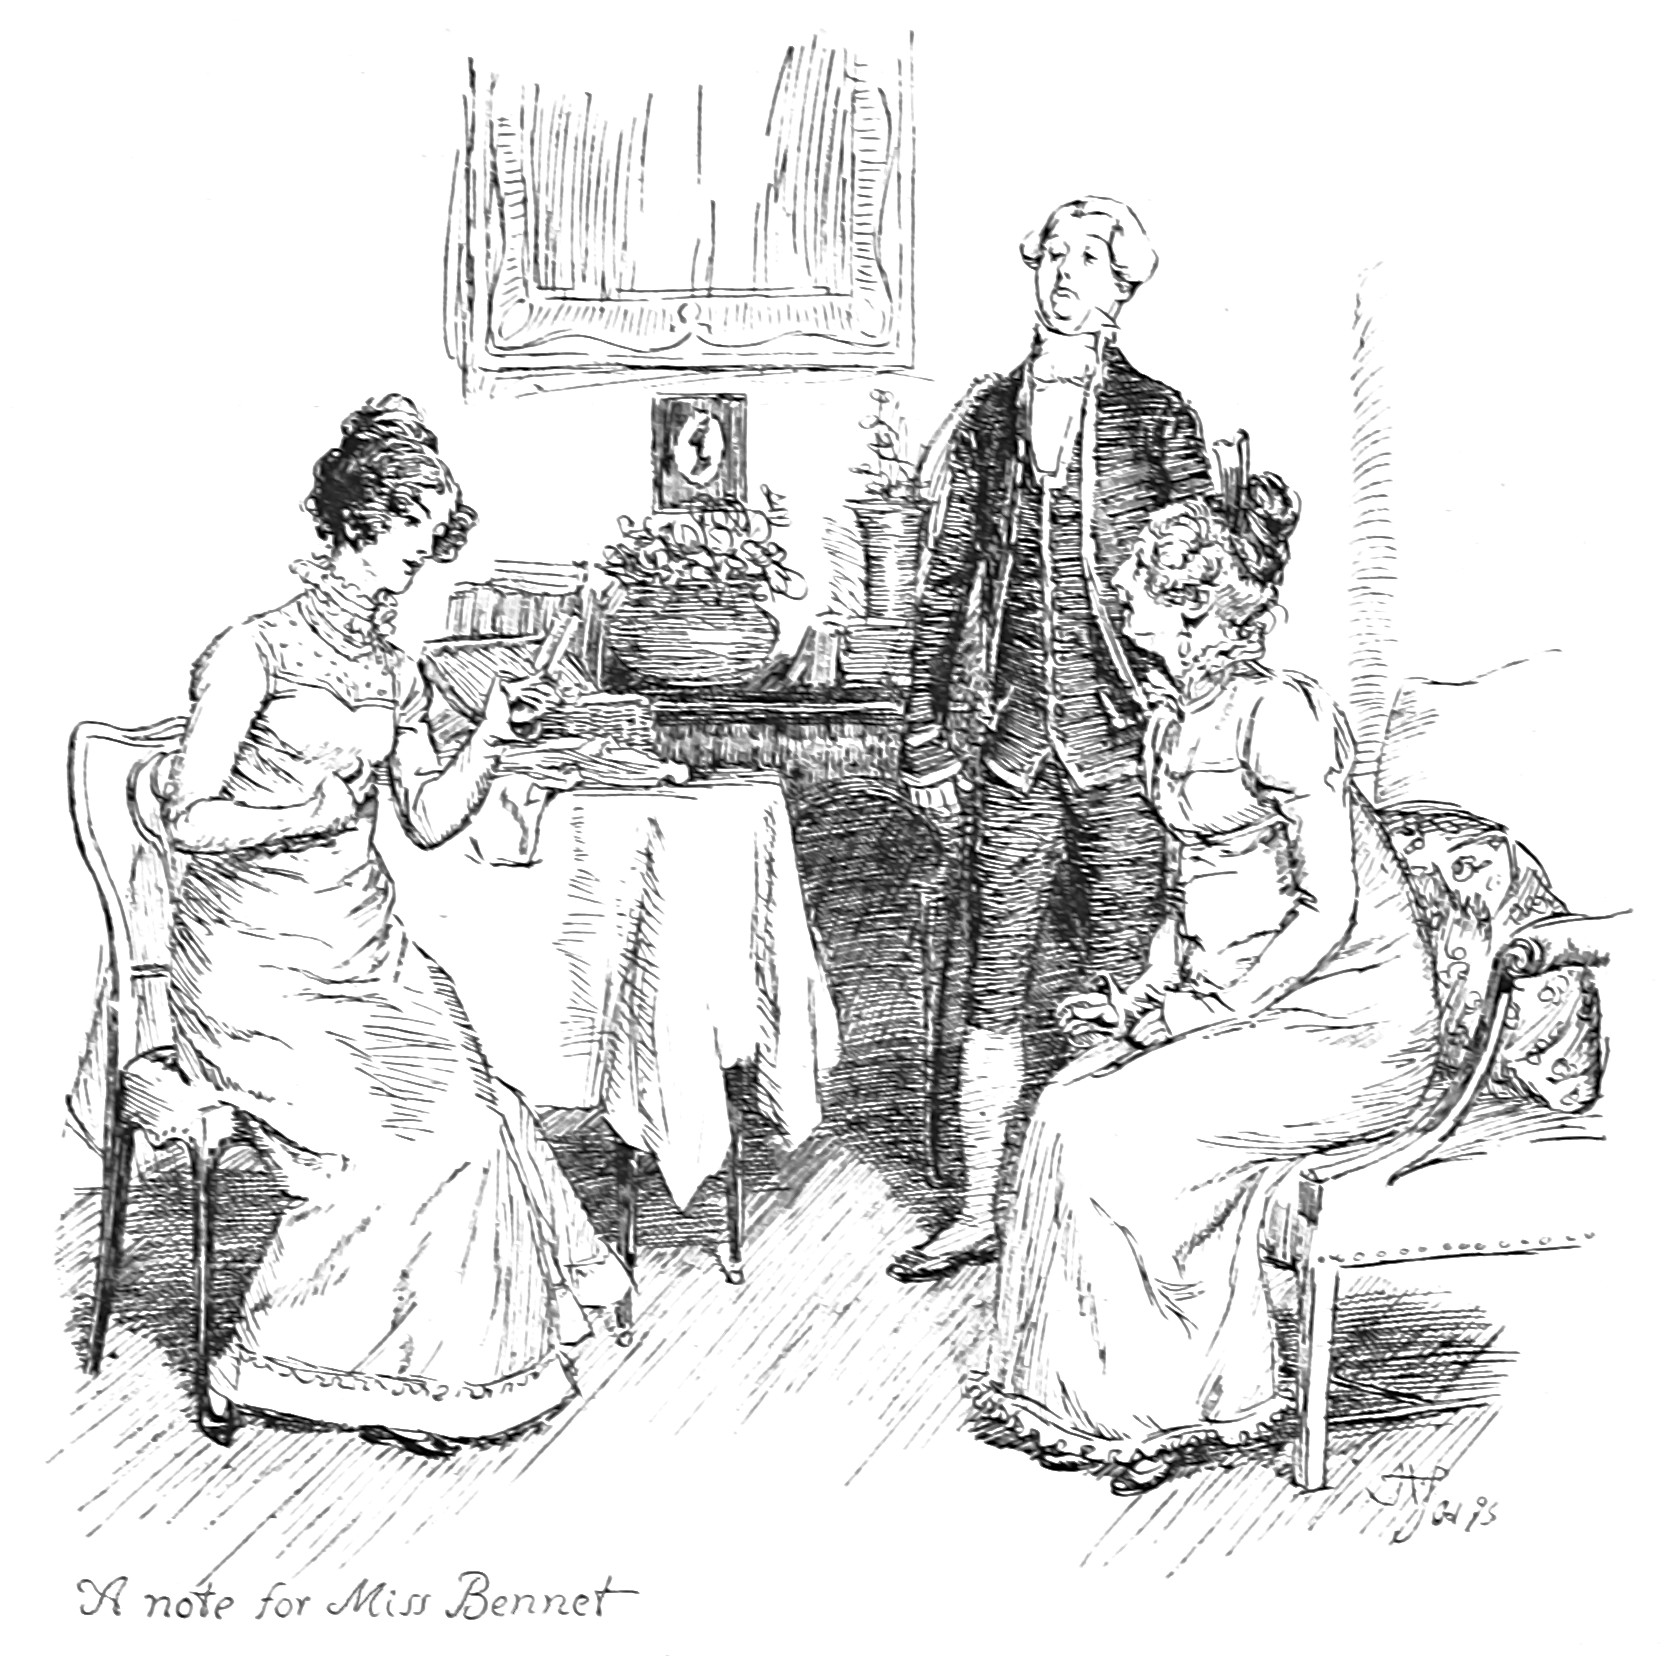
\includegraphics[width=.8\linewidth]{7note}
\captionlistentry{A note for Miss Bennet}
\end{figure}

\lettrine[lines=6,image=true]{initials/chap7m}{r}  Bennet's property consisted almost entirely in an estate of two thousand a year, which, unfortunately for his daughters, was entailed, in default of heirs male, on a distant relation; and their mother's fortune, though ample for her situation in life, could but ill supply the deficiency of his. Her father had been an attorney in Meryton, and had left her four thousand pounds.

She had a sister married to a Mr Philips, who had been a clerk to their father and succeeded him in the business, and a brother settled in London in a respectable line of trade.

The village of Longbourn was only one mile from Meryton; a most convenient distance for the young ladies, who were usually tempted thither three or four times a week, to pay their duty to their aunt, and to a milliner's shop just over the way. The two youngest of the family, Catherine and Lydia, were particularly frequent in these attentions: their minds were more vacant than their sisters', and when nothing better offered, a walk to Meryton was necessary to amuse their morning hours and furnish conversation for the evening; and, however bare of news the country in general might be, they always contrived to learn some from their aunt. At present, indeed, they were well supplied both with news and happiness by the recent arrival of a militia regiment in the neighbourhood; it was to remain the whole winter, and Meryton was the head-quarters.

Their visits to Mrs Philips were now productive of the most interesting intelligence. Every day added something to their knowledge of the officers' names and connections. Their lodgings were not long a secret, and at length they began to know the officers themselves. Mr Philips visited them all, and this opened to his nieces a source of felicity unknown before. They could talk of nothing but officers; and Mr Bingley's large fortune, the mention of which gave animation to their mother, was worthless in their eyes when opposed to the regimentals of an ensign.

After listening one morning to their effusions on this subject, Mr Bennet coolly observed,—

»From all that I can collect by your manner of talking, you must be two of the silliest girls in the country. I have suspected it some time, but I am now convinced.«

Catherine was disconcerted, and made no answer; but Lydia, with perfect indifference, continued to express her admiration of Captain Carter, and her hope of seeing him in the course of the day, as he was going the next morning to London.

»I am astonished, my dear,« said Mrs Bennet, »that you should be so ready to think your own children silly. If I wished to think slightingly of anybody's children, it should not be of my own, however.«

»If my children are silly, I must hope to be always sensible of it.«

»Yes; but as it happens, they are all of them very clever.«

»This is the only point, I flatter myself, on which we do not agree. I had hoped that our sentiments coincided in every particular, but I must so far differ from you as to think our two youngest daughters uncommonly foolish.«

»My dear Mr Bennet, you must not expect such girls to have the sense of their father and mother. When they get to our age, I dare say they will not think about officers any more than we do. I remember the time when I liked a red coat myself very well—and, indeed, so I do still at my heart; and if a smart young colonel, with five or six thousand a year, should want one of my girls, I shall not say nay to him; and I thought Colonel Forster looked very becoming the other night at Sir William's in his regimentals.«

»Mamma,« cried Lydia, »my aunt says that Colonel Forster and Captain Carter do not go so often to Miss Watson's as they did when they first came; she sees them now very often standing in Clarke's library.«

Mrs Bennet was prevented replying by the entrance of the footman with a note for Miss Bennet; it came from Netherfield, and the servant waited for an answer. Mrs Bennet's eyes sparkled with pleasure, and she was eagerly calling out, while her daughter read,—

»Well, Jane, who is it from? What is it about? What does he say? Well, Jane, make haste and tell us; make haste, my love.«

»It is from Miss Bingley,« said Jane, and then read it aloud.

%\pagebreak[4]

\begin{samepage}
\begin{quotation}
\noindent My dear friend,\\

\indent If you are not so compassionate as to dine to-day with Louisa and me, we shall be in danger of hating each other for the rest of our lives; for a whole day's \textit{tête-à-tête} between two women can never end without a quarrel. Come as soon as you can on the receipt of this. My brother and the gentlemen are to dine with the officers. \\

\begin{flushright}
Yours ever,\\
\textsc{Caroline Bingley.}
\end{flushright}
\end{quotation}
\end{samepage}
%\enlargethispage{\baselineskip}

»With the officers!« cried Lydia: »I wonder my aunt did not tell us of \textit{that}.«

»Dining out,« said Mrs Bennet; »that is very unlucky.«

»Can I have the carriage?« said Jane.

»No, my dear, you had better go on horseback, because it seems likely to rain; and then you must stay all night.«

»That would be a good scheme,« said Elizabeth, »if you were sure that they would not offer to send her home.«

»Oh, but the gentlemen will have Mr Bingley's chaise to go to Meryton; and the Hursts have no horses to theirs.«

»I had much rather go in the coach.«

»But, my dear, your father cannot spare the horses, I am sure. They are wanted in the farm, Mr Bennet, are not they?«


»They are wanted in the farm much oftener than I can get them.«

»But if you have got them to-day,« said Elizabeth, »my mother's purpose will be answered.«

\begin{a4}
	\begin{figure}[tbh]
	\centering
	
\includegraphics[width=.7\linewidth]{7cheerful}
	\captionlistentry{Cheerful prognostics}
	\end{figure}
\end{a4}

She did at last extort from her father an acknowledgment that the horses were engaged; Jane was therefore obliged to go on horseback, and her mother attended her to the door with many cheerful prognostics of a bad day. Her hopes were answered; Jane had not been gone long before it rained hard. Her sisters were uneasy for her, but her mother was delighted. The rain continued the whole evening without intermission; Jane certainly could not come back.

»This was a lucky idea of mine, indeed!« said Mrs Bennet, more than once, as if the credit of making it rain were all her own. Till the next morning, however, she was not aware of all the felicity of her contrivance. Breakfast was scarcely over when a servant from Netherfield brought the following note for Elizabeth:—

%\pagebreak[4]

\begin{samepage}
\begin{quotation}
\noindent My dearest Lizzie,\\

\indent I find myself very unwell this morning, which, I suppose, is to be imputed to my getting wet through yesterday. My kind friends will not hear of my returning home till I am better. They insist also on my seeing Mr Jones—therefore do not be alarmed if you should hear of his having been to me—and, excepting a sore throat and a headache, there is not much the matter with me.\\

\begin{flushright}
\noindent Yours, etc.
\end{flushright}
\end{quotation}
\end{samepage}



»Well, my dear,« said Mr Bennet, when Elizabeth had read the note aloud, »if your daughter should have a dangerous fit of illness—if she should die—it would be a comfort to know that it was all in pursuit of Mr Bingley, and under your orders.«

»Oh, I am not at all afraid of her dying. People do not die of little trifling colds. She will be taken good care of. As long as she stays there, it is all very well. I would go and see her if I could have the carriage.«

Elizabeth, feeling really anxious, determined to go to her, though the carriage was not to be had: and as she was no horsewoman, walking was her only alternative. She declared her resolution.

»How can you be so silly,« cried her mother, »as to think of such a thing, in all this dirt! You will not be fit to be seen when you get there.«

»I shall be very fit to see Jane—which is all I want.«

»Is this a hint to me, Lizzy,« said her father, »to send for the horses?«

»No, indeed. I do not wish to avoid the walk. The distance is nothing, when one has a motive; only three miles. I shall be back by dinner.«

\begin{letter}
	\begin{figure}[tbh]
	\centering
	
\includegraphics[width=.7\linewidth]{7cheerful}
	\captionlistentry{Cheerful prognostics}
	\end{figure}
\end{letter}

»I admire the activity of your benevolence,« observed Mary, »but every impulse of feeling should be guided by reason; and, in my opinion, exertion should always be in proportion to what is required.«

»We will go as far as Meryton with you,« said Catherine and Lydia. Elizabeth accepted their company, and the three young ladies set off together.



»If we make haste,« said Lydia, as they walked along, »perhaps we may see something of Captain Carter, before he goes.«

In Meryton they parted: the two youngest repaired to the lodgings of one of the officers' wives, and Elizabeth continued her walk alone, crossing field after field at a quick pace, jumping over stiles and springing over puddles, with impatient activity, and finding herself at last within view of the house, with weary ancles, dirty stockings, and a face glowing with the warmth of exercise.

%\begin{wrapfigure}{O}{0.5\textwidth}
	\begin{figure}[bh]
\centering
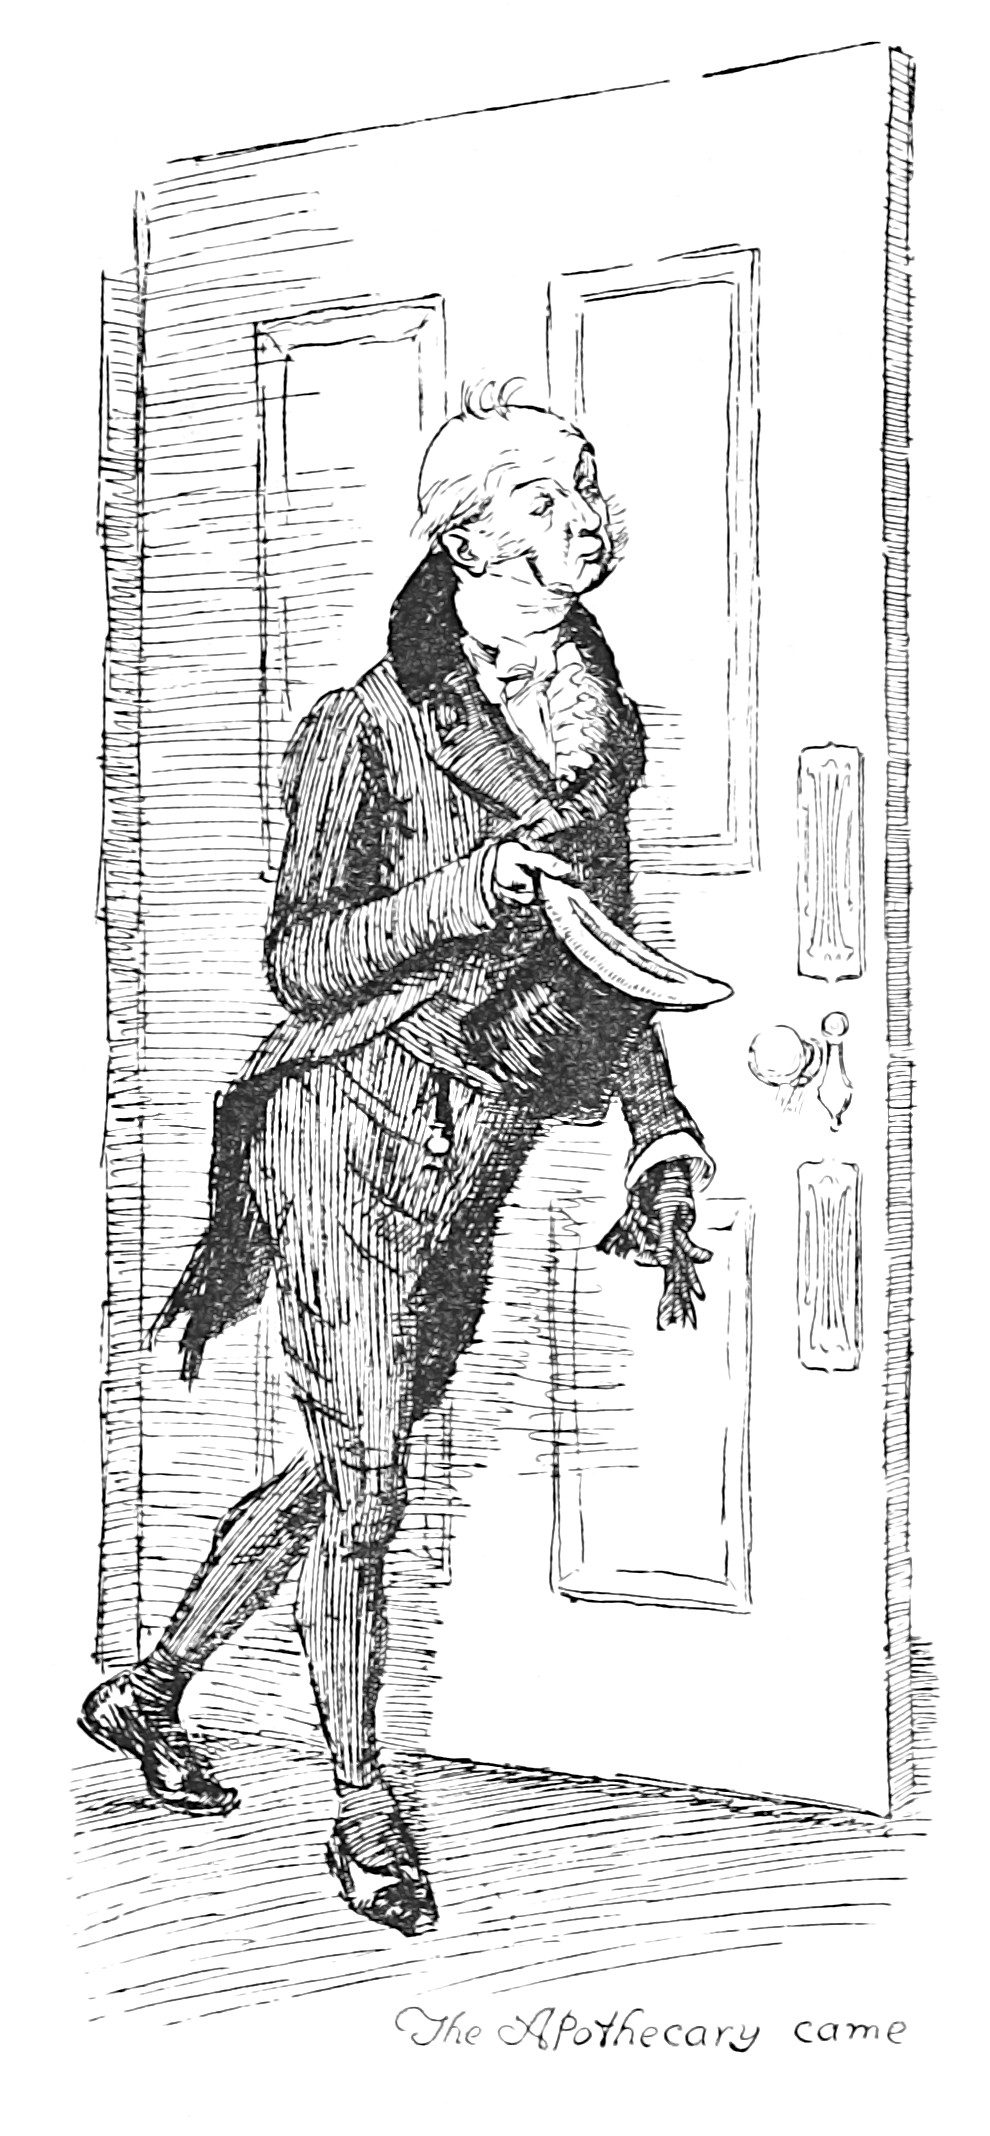
\includegraphics[width=0.35\textwidth]{7apothecary}
\captionlistentry{The apothecary came}
\end{figure}
%\end{wrapfigure}

She was shown into the breakfast parlour, where all but Jane were assembled, and where her appearance created a great deal of surprise. That she should have walked three miles so early in the day in such dirty weather, and by herself, was almost incredible to Mrs Hurst and Miss Bingley; and Elizabeth was convinced that they held her in contempt for it. She was received, however, very politely by them; and in their brother's manners there was something better than politeness—there was good-humour and kindness. Mr Darcy said very little, and Mr Hurst nothing at all. The former was divided between admiration of the brilliancy which exercise had given to her complexion and doubt as to the occasion's justifying her coming so far alone. The latter was thinking only of his breakfast.

%\clearpage



Her inquiries after her sister were not very favourably answered. Miss Bennet had slept ill, and though up, was very feverish, and not well enough to leave her room. Elizabeth was glad to be taken to her immediately; and Jane, who had only been withheld by the fear of giving alarm or inconvenience, from expressing in her note how much she longed for such a visit, was delighted at her entrance. She was not equal, however, to much conversation; and when Miss Bingley left them together, could attempt little beside expressions of gratitude for the extraordinary kindness she was treated with. Elizabeth silently attended her.



When breakfast was over, they were joined by the sisters; and Elizabeth began to like them herself, when she saw how much affection and solicitude they showed for Jane. The apothecary came; and having examined his patient, said, as might be supposed, that she had caught a violent cold, and that they must endeavour to get the better of it; advised her to return to bed, and promised her some draughts. The advice was followed readily, for the feverish symptoms increased, and her head ached acutely. Elizabeth did not quit her room for a moment, nor were the other ladies often absent; the gentlemen being out, they had in fact nothing to do elsewhere.

When the clock struck three, Elizabeth felt that she must go, and very unwillingly said so. Miss Bingley offered her the carriage, and she only wanted a little pressing to accept it, when Jane testified such concern at parting with her that Miss Bingley was obliged to convert the offer of the chaise into an invitation to remain at Netherfield for the present. Elizabeth most thankfully consented, and a servant was despatched to Longbourn, to acquaint the family with her stay, and bring back a supply of clothes.